% Created 2019-10-03 Thu 21:53
% Intended LaTeX compiler: pdflatex
\documentclass[11pt]{article}
\usepackage[utf8]{inputenc}
\usepackage[T1]{fontenc}
\usepackage{graphicx}
\usepackage{grffile}
\usepackage{longtable}
\usepackage{wrapfig}
\usepackage{rotating}
\usepackage[normalem]{ulem}
\usepackage{amsmath}
\usepackage{textcomp}
\usepackage{amssymb}
\usepackage{capt-of}
\usepackage{hyperref}
\usepackage[left=1in,top=1in,right=1in,bottom=1.5in]{geometry}
\usepackage{palatino}
\usepackage{fancyhdr}
\usepackage{sectsty}
\usepackage{engord}
\usepackage{cite}
\usepackage{graphicx}
\usepackage{setspace}
\usepackage[center]{caption}
\usepackage{multirow}
\usepackage{ifthen}
\usepackage{longtable}
\usepackage{color}
\usepackage{amsmath}
\usepackage{listings}
\usepackage{pdfpages}
\usepackage{nomencl}	% For glossary
\usepackage{pdflscape}	% For landscape pictures and environment
\usepackage{verbatim}   % For multiline comment environments
\usepackage[table]{xcolor}
\author{Group 5}
\date{\today}
\title{ISP Project Internet Services}
\hypersetup{
 pdfauthor={Group 5},
 pdftitle={ISP Project Internet Services},
 pdfkeywords={},
 pdfsubject={},
 pdfcreator={Emacs 26.1 (Org mode 9.1.1)},
 pdflang={English}}
\begin{document}

\maketitle
\setlength\parindent{0pt}

\section{Virtualbox VM Config}
\label{sec:orga77be60}

\subsection{Host IP Config}
\label{sec:org7fc3342}

First config host \emph{your computer} and set a static ip address \texttt{10.5.5.10} that belongs to the server network \texttt{10.5.5.0/24}

The static ip address \textbf{has to} be set onto the interface that the ethernet cable connecting to e.g. \texttt{en1: Thunderbold 1}.

\begin{figure}[htbp]
\centering
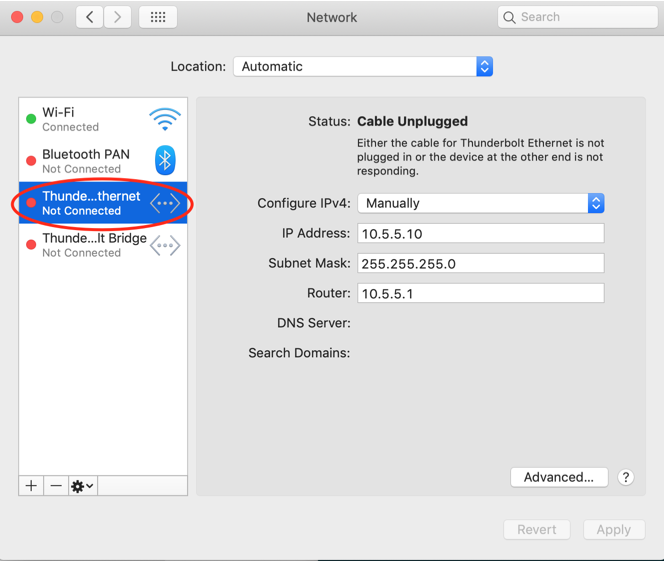
\includegraphics[width=.9\linewidth]{./img/host.png}
\caption{set a static ip address on a mac computer}
\end{figure}

From the host verify that you can \texttt{ping} RTB (\emph{Router B} \texttt{ping 10.5.5.1}.

\subsection{VM IP Config}
\label{sec:orgdaedea8}

Before starting your VM on Virtualbox, you need to config VM \textbf{Network} to use \textbf{Bridged Adpater} and make sure:

\begin{itemize}
\item \textbf{attach to} the interface that has ethernet cable connected. e.g. \texttt{en1: Thunderbold 1}.
\item set Promiscuous Mode: Allow All
\end{itemize}

\begin{figure}[htbp]
\centering
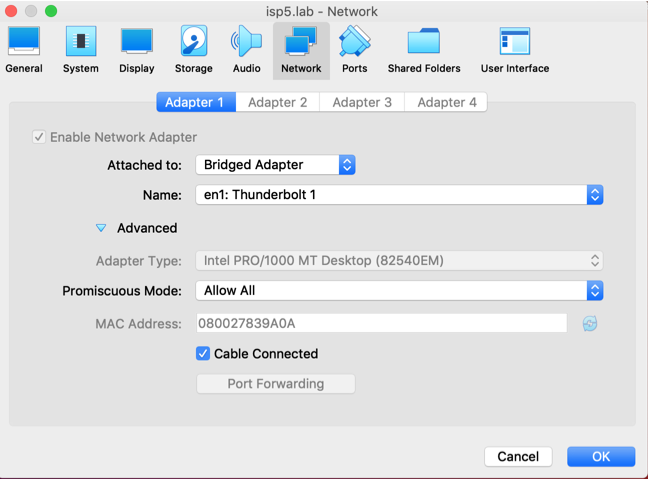
\includegraphics[width=.9\linewidth]{./img/vm.png}
\caption{virtualbox network adaptor}
\end{figure}

Now start the VM.

\begin{enumerate}
\item Install \texttt{net-tools} package.

\begin{verbatim}
sudo apt install net-tools
sudo apt install vim # only if you use vim editor
\end{verbatim}

\item Edit \texttt{/etc/network/interfaces}.

Replace its content with the lines below. This will set a static ip \texttt{10.5.5.5} to the VM.

As a note the interface name e.g. \texttt{ens3} must match, you can find the interface name through command \texttt{ifconfig}

\begin{verbatim}
auto lo
iface lo inet loopback

auto ens3
iface ens3 inet static
address 10.5.5.5
netmask 255.255.255.0
\end{verbatim}

\item Restart \texttt{networking} and reboot VM

\begin{verbatim}
sudo systemctl restart networking
reboot
\end{verbatim}

\item Verify

\begin{itemize}
\item verify that you can \texttt{ping} your host from VM. \texttt{ping 10.5.5.10}
\item veriy that you can \texttt{ping} the router from VM. \texttt{ping 10.5.5.1}
\end{itemize}
\end{enumerate}

\subsection{Set default gateway to RTB}
\label{sec:orgd3c5bf1}

\begin{verbatim}
sudo route set default gateway 10.5.5.1
route -n
\end{verbatim}

Verify that you can reach client network \texttt{ping 10.5.10.1}

\section{DHCP config}
\label{sec:org6725509}

\subsection{Install isc-dhcp-server}
\label{sec:org446a426}

\begin{verbatim}
sudo apt update
sudo apt install isc-dhcp-server
\end{verbatim}

\subsection{Config interface that dhcp server listens on}
\label{sec:orgcca5f04}

\begin{enumerate}
\item Run command \texttt{ifconfig} and take note of the interface name that has ip address \texttt{10.5.5.5}, e.g. \texttt{enp0s3}
\item Edit \texttt{/etc/default/isc-dhcp-server} file to set the interface name.
\begin{verbatim}
INTERFACESv4="enp0s3"
INTERFACESv6=""
\end{verbatim}
\end{enumerate}

\subsection{Config dhcp server}
\label{sec:org3ddb907}

\begin{enumerate}
\item Edit the main dhcp configuration file \texttt{/etc/dhcp/dhcpd.conf} and add the lines below:

\begin{verbatim}
option domain-name "isp5.lab";
option domain-name-servers 10.5.5.5;

default-lease-time 600;
max-lease-time 7200;

ddns-update-style none;

authoritative;

## config the subnet for server network
subnet 10.5.5.0 netmask 255.255.255.0 {
  range 10.5.5.100 10.5.5.200
  option domain-name-servers 10.5.5.5;
  option domain-name "isp5.lab";
  option subnet-mask 255.255.255.0;
  option routers 10.5.5.1;
  option broadcast-address 10.5.5.255;
  default-lease-time 600;
  max-lease-time 7200;
}

## config the subnet for client network
subnet 10.5.10.0 netmask 255.255.255.0 {
  range 10.5.10.100 10.5.10.200
  option domain-name-servers 10.5.5.5;
  option domain-name "isp5.lab";
  option subnet-mask 255.255.255.0;
  option routers 10.5.10.1;
  option broadcast-address 10.5.10.255;
  default-lease-time 600;
  max-lease-time 7200;
}
\end{verbatim}

\item Start dhcp server
\begin{verbatim}
sudo systemctl start isc-dhcp-server
# or
sudo server isc-dhcp-server start
\end{verbatim}

\item Verify dhcp server status
\begin{verbatim}
sudo systemctl status isc-dhcp-server
\end{verbatim}
\end{enumerate}

\subsubsection{Troublshooting}
\label{sec:orgab1f322}

if server status is not \textbf{active}, check the error logs by running command \texttt{view /var/log/syslog}.
And press \texttt{SHIFT + g} to scroll to the bottom of the file.

After having fixed the issue, restart dhcp server and verify status again.

\subsection{Install DHCP Relay on Router C}
\label{sec:orgbad5548}

\begin{verbatim}
enable
config terminal
interface Gi 0/1

ip address-helper 10.5.5.5
do wr
\end{verbatim}

\subsection{Verify}
\label{sec:orgb0c491a}

Once the DHCP server is up and running and DHCP relay is installed on Router C,
you can connect another computer to the client network and run the following command to verify.

\begin{verbatim}
sudo route add default gateway 10.5.10.1
sudo dhclient eth1
ifconfig # check if you got ip address between 10.5.10.100 and 10.5.10.200 on interface eth1.
\end{verbatim}

\texttt{eth1} needs to be replaced with the actual client interface name.


\section{Bind9 DNS Config}
\label{sec:orga01fd8a}

\subsection{Install bind9, bin9utils}
\label{sec:orgfa0d93c}

\begin{verbatim}
sudo apt update
sudo apt install bind9 bin9utils
\end{verbatim}

\subsection{Edit \texttt{/etc/bind/named.conf.local} file.}
\label{sec:org3dbb4ed}

\texttt{sudo vim /etc/bind/named.conf.local} and add zones configuration:

\begin{verbatim}
zone "isp5.lab" { type master; file "/etc/bind/db.isp5.lab"; };
zone "5.5.10.in-addr.arpa" { type master; file "/etc/bind/db.10.5.5"; };
\end{verbatim}

Run the command \texttt{sudo named-checkconf -z /etc/bind/named.conf} to validate.

\subsection{Create a file at \texttt{/etc/bind/db.isp5.lab}}
\label{sec:org4443ebe}

First copy \texttt{/etc/bind/db.local/}:

\begin{verbatim}
sudo cp /etc/bin/db.local /etc/bind/db.isp5.lab
\end{verbatim}

First replace the settings that has  \texttt{localhost.}, \texttt{root.localhost.} to \texttt{isp5.lab}, \texttt{root.isp5.lab.}

\begin{itemize}
\item \textbf{DO NOT forget} the 'dot'/'.' in the end
\item \textbf{MUST increament the serial number:} \texttt{2     ; Serial}, every time you make changes this file
\end{itemize}

\begin{center}
\begin{tabular}{lllll}
@ & IN & SOA & localhost. & root.localhost.\\
\end{tabular}
\end{center}
Change to
\begin{center}
\begin{tabular}{lllll}
@ & IN & SOA & isp5.lab. & root.isp5.lab.\\
\end{tabular}
\end{center}

Then update the settings:

\begin{center}
\begin{tabular}{lllr}
@ & IN & NS & ns.isp5.lab\\
@ & IN & A & 10.5.5.5\\
ns & IN & A & 10.5.5.5\\
dhcpd & IN & CNAME & ns\\
www & IN & CNAME & ns\\
client1 & IN & A & 10.5.10.100\\
client2 & IN & A & 10.5.10.101\\
\end{tabular}
\end{center}

Run the command \texttt{sudo named-checkzone forward /etc/bind/db.isp5.lab} to validate.

\subsection{Create a file at \texttt{/etc/bind/db.10.5.5}}
\label{sec:org0b9a174}

First copy \texttt{/etc/bind/db.isp5.lab}

\begin{verbatim}
sudo cp /etc/bind/db.isp5.lab /etc/bind/db.10.5.5
\end{verbatim}

And update the settings:

\begin{center}
\begin{tabular}{rlll}
@ & IN & NS & ns.isp5.lab.\\
5 & IN & PTR & ns.isp5.lab.\\
100 & IN & PTR & client1.isp5.lab.\\
101 & IN & PTR & client2.isp5.lab.\\
\end{tabular}
\end{center}

\textbf{The serial number in the reverse zone needs to be incremented on each changes as well}

Run the command \texttt{sudo named-checkzone reverse /etc/bind/db.10.5.5} to validate.

\subsection{Start bind9}
\label{sec:orgb60d7c9}

Start \texttt{bind9} service
\begin{verbatim}
sudo chown -R bind:bind /etc/bind
sudo chmod -R 755 /etc/bind

sudo systemctl start bind9
\end{verbatim}

\subsection{Check status}
\label{sec:org952ee8e}
Check \texttt{bind9} service status
\begin{verbatim}
sudo systemctl status bind9
\end{verbatim}

\subsubsection{Troubleshooting}
\label{sec:org0912d3e}
if server status is not \textbf{active}, check the error logs by running command \texttt{view /var/log/syslog}.
And press \texttt{SHIFT + g} to scroll to the bottom of the file.

After having fixed the issue, restart bind9 server and very status again.

\subsection{Config \texttt{/etc/network/interfaces} file}
\label{sec:org78ffa3c}

\begin{enumerate}
\item Edit \texttt{/etc/network/interfaces} file and add the lines below

\begin{verbatim}
dns-search isp5.lab
dns-nameserver 10.5.5.5
\end{verbatim}

\item Restart networking device:

\begin{verbatim}
sudo systemctl restart networking
\end{verbatim}
\end{enumerate}

\subsection{Config \texttt{/etc/resolv.conf} file}
\label{sec:org9fda2dd}

\begin{enumerate}
\item Edit \texttt{/etc/resolv.conf} file and add the lines below

\begin{verbatim}
nameserver 10.5.5.5
search isp5.lab
\end{verbatim}

\item Restart networking and NetworkManager
\begin{verbatim}
sudo systemctl restart networking
sudo systemctl restart NetWorkManager

## Maybe restart bind9?
sudo systemctl restart bind9
\end{verbatim}
\end{enumerate}

\subsection{Verify with \texttt{ping} and \texttt{nslookup}}
\label{sec:org07c3c5b}

\begin{verbatim}
ping ns
ping client1

nslookup ns
nslookup client1
\end{verbatim}


\subsection{client side}
\label{sec:org4ee7255}

\textbf{NOTE} The following configuration should be auto fixed when client receives an ip address from DHCP server

\begin{enumerate}
\item Edit /etc/network/interfaces
\texttt{sudo vim /etc/network/interfaces} and add the following lines:

\begin{verbatim}
dns-search isp5.lab
dns-nameserver 10.5.5.5
\end{verbatim}

\item Edit /etc/resolv.conf
\texttt{sudo vim /etc/resolv.conf} and add the followling lines:

\begin{verbatim}
nameserver 10.5.5.5
search 10.5.5.5
\end{verbatim}

\item Restart netwoking and NetworkManager

\begin{verbatim}
sudo systemctl restart networking
sudo systemctl restart NetWorkManager

ping 10.5.5.5
\end{verbatim}
\end{enumerate}


\section{Nginx Config}
\label{sec:orgbecf9ed}

\subsection{Install Nginx}
\label{sec:org609a997}

\begin{verbatim}
sudo apt install nginx
\end{verbatim}

\subsubsection{Verify nginx is running}
\label{sec:orgffdbee5}
\begin{verbatim}
service nginx status
\end{verbatim}

Now go to \url{http://localhost:80} on Firefox in your VM where Nginx is installed.

\subsection{Config}
\label{sec:org444f7d6}

\begin{enumerate}
\item Run \texttt{less /etc/nginx/sites-available/default} to check where \texttt{index.html} is located.
And Press \texttt{q} to exit.
\begin{verbatim}
server {
  listen 80 default_server;
  ....
  root /var/www/html
  index index.html index.htm, index.nginx-debian.html.back
}
\end{verbatim}

\item Run the commands below to create a new file \texttt{index.html}
\end{enumerate}

\begin{verbatim}
sudo cp /var/www/html/index.nginx-debian.html /var/www/htm/index.nginx-debian.html.back
sudo mv /var/www/htm/index.nginx-debian.html /var/www/html/index.html
\end{verbatim}

\begin{enumerate}
\item Edit \texttt{index.html} file

\begin{verbatim}
sudo vim /var/www/html/index.html
\end{verbatim}

\item Refresh firefox at \url{http://localhost:80}
\end{enumerate}

\subsection{Common commands}
\label{sec:org285490f}

\begin{verbatim}
service nginx help
\end{verbatim}
\end{document}